\section{Tổng quan hệ thống}

\subsection{Trò chơi Bloxorz}

Người chơi lăn một khối hộp 1×1×2 trên một bàn gồm các ô vuông lơ lửng để đưa khối \textbf{đứng thẳng} vào lỗ đích. Khối có ba tư thế: đứng, nằm ngang và nằm dọc. Khối rơi khỏi bàn (thua) nếu có phần nào nằm ngoài bàn hoặc trên ô trống. Ngoài sàn thường, bàn có thể có ô dễ vỡ, cầu đóng/mở được, và ba loại công tắc: công tắc mềm, công tắc nặng và công tắc tách khối thành hai khối lập phương 1×1×1. Luật chi tiết của từng loại ô được trình bày cùng mô hình chuyển trạng thái ở mục 3.4.

\subsection{Kiến trúc mã nguồn}

{\renewcommand{\arraystretch}{1.25}
\begin{longtable}{|>{\raggedright\arraybackslash}p{0.199\linewidth}|>{\raggedright\arraybackslash}p{0.731\linewidth}|}
\hline
\textbf{Mô-đun} & \textbf{Vai trò} \\ \hline
\endhead
\texttt{bloxorz/core} & Trạng thái, bảng chuyển tư thế, luật ô đặc biệt, bộ đọc màn JSON, giao diện bài toán \texttt{BloxorzProblem} \\ \hline
\texttt{bloxorz/solvers} & BFS, DFS, IDS, UCS, A*; hàm chi phí; heuristic; mô-đun đo hiệu năng \\ \hline
\texttt{bloxorz/gui} & Giao diện Pygame: vẽ bàn và khối, điều khiển, chạy solver, phát lại lời giải \\ \hline
\texttt{benchmark} & Chạy thực nghiệm, sinh bảng và biểu đồ \\ \hline
\texttt{levels} & 16 màn chơi JSON thuộc 4 nhóm độ khó \\ \hline
\end{longtable}
}

Phần lõi và phần thuật toán không phụ thuộc vào giao diện. Mọi thuật toán dùng chung một chữ ký gọi hàm và cùng trả về \texttt{SearchResult} gồm đường đi (danh sách hành động, hoặc \texttt{None} nếu không có lời giải) và bộ bốn số liệu: thời gian tìm kiếm, bộ nhớ đỉnh, số nút mở rộng và độ dài lời giải. Sơ đồ 1 mô tả luồng xử lý từ tệp màn chơi đến bảng số liệu trong báo cáo.

\begin{sodo}[H]
\centering
\caption{Quy trình xử lý tổng thể của hệ thống}
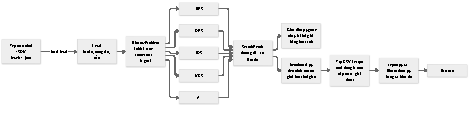
\includegraphics[width=\linewidth,height=0.78\textheight,keepaspectratio]{images/sodo1.pdf}
\end{sodo}

\subsection{Giao diện đồ hoạ}

\begin{itemize}
\item \textbf{Điều khiển:} phím mũi tên hoặc W/A/S/D để lăn khối; phím Space để đổi khối được điều khiển khi đang tách; phím R để chơi lại màn.
\item \textbf{Nút bấm:} \texttt{\textless{} Prev} / \texttt{Next \textgreater{}} (chọn màn), \texttt{New Game}, \texttt{Restart}, và bốn nút \texttt{Solve BFS}, \texttt{Solve DFS}, \texttt{Solve UCS}, \texttt{Solve A*}.
\item \textbf{Chạy solver:} thuật toán chạy trên một luồng riêng nên giao diện không bị treo. Khi có kết quả, lời giải được phát lại bằng hoạt ảnh lăn khối, và bảng \emph{Solver Metrics} hiển thị tên thuật toán, độ dài lời giải, số nút mở rộng, thời gian tìm kiếm và cost của lời giải.
\end{itemize}
